\documentclass[t,aspectratio=169]{beamer}



\author{William O'Mullane}
\institute{AURA/Rubin Observatory}
\title{LSST Data Management }
\date{  \today}


\graphicspath{ {./images/} {./ETCcharts/} }

\def\pasp{PASP}

\usepackage{pdfpages}
\usepackage{amsmath,graphicx,marvosym}
\usepackage{tikz,multirow,array,colortbl,multimedia}
\usepackage{times,layouts}
\usepackage{tikz,hyperref}
\usetikzlibrary{positioning,arrows,shapes,decorations.shapes,shapes.arrows}
\usetikzlibrary{backgrounds,calc, shadows}
\usetikzlibrary{shapes.callouts}

\usepackage{graphicx}
\usepackage{natbib}
\usepackage{longtable}

\tikzstyle{flow}=[->, >=stealth', thick, shorten >=3pt, shorten <=3pt]

\def\aaps{A\&AS}           % Astronomy and Astrophysics Suplement
\def\aap{A\&A}             % Astronomy and Astrophysics
\def\ssr{Space~Sci.~Rev.}  % Space Science Reviews
\def\apj{ApJ}              % Astrophysical Journal
\def\aj{AJ}                % Astronomical Journal
\def\mnras{MNRAS}          % Monthly Notices of the RAS
\def\araa{ARA\&A}          % Annual Review of Astron and Astrophys
\def\nat{Nature}           % Nature
\def\apjl{ApJ}             % Astrophysical Journal, Letters

\def\degr{\hbox{$^\circ$}}
\def\arcmin{\hbox{$^\prime$}}
\def\arcsec{\hbox{$^{\prime\prime}$}}
\def\fs{\hbox{$.\!\!^{\rm s}$}}
\def\fdg{\hbox{$.\!\!^\circ$}}
\def\farcm{\hbox{$.\mkern-4mu^\prime$}}
\def\farcs{\hbox{$.\!\!^{\prime\prime}$}}
\def\sun{\hbox{$\odot$}}


%\newcommand{\bfvec}[1]{\mbox{$\bf#1$}}
%\newcommand{\citell}{\citeyear}
\newcommand{\citeds}{\citeyear}
%\newcommand{\citellp}{\citeyearpar}
%\newcommand{\citedsp}{\citeyearpar}
\providecommand{\secref}[1]{Section~\ref{#1}}
\providecommand{\appref}[1]{Appendix~\ref{#1}}
\providecommand{\partref}[1]{Part~\ref{#1}}
\providecommand{\tabref}[1]{Table~\ref{#1}}
\providecommand{\figref}[1]{Figure~\ref{#1}}
\providecommand{\eqnref}[1]{Eq.~\ref{#1}}
\providecommand{\reqref}[1]{Req.~\ref{#1}}
\providecommand{\actref}[1]{AI~\ref{#1}}


\newcommand{\jira}[1]{\href{https://jira.lsstcorp.org/browse/#1}{#1}}


\usepackage[fonts=false, footline={William O'Mullane \hfill LSST DM  \hfill},
meeting={LSP Observatory Review 2017},
position={DM Project Manager}
]{LSST-beamer}

\author{William O'Mullane  {\tiny input from \u{Z}eljko Ivezi\'c }}
\date{Paranal  13$^{th}$  December 2017}
\title{LSST Data Mangement}

\begin{document}

\maketitle


\frame{\frametitle{The History of LSST }
\vspace{-10pt}
\center {\large \color{blue} A New Kind of Telescope Optimized for Surveys  }
\vspace{5pt}
\begin{columns}
\column{0.33\textwidth}
{\color{red}$\sim$2000}\\
\vspace{5pt}
Modified 3-mirror Paul-Baker Design
Seeing limited over 3.5 deg field of view
{\em Dark Matter Telescope}
\\
\includegraphics[width=0.6\textwidth]{images/2kDesign}

\column{0.33\textwidth}
{\color{red} $\sim$2010}\\
\vspace{5pt}
LSST selected as the highest priority ground-based instrument for the coming decade
\\
\includegraphics[width=0.4\textwidth]{images/newHorizons}

\column{0.33\textwidth}
{\color{red} $\sim$2014}\\
\vspace{5pt}
Formal construction start!\\
Joint DOE + NSF project
\\
\vspace{20pt}
\includegraphics[width=0.8\textwidth]{images/LSSTconstStart}\\

\vspace {1cm}
{\tiny \bf Beth Willman}
\end{columns}

}

\frame { \frametitle{ LSST:uniform sky survey }
\begin{columns}
\column{0.45\textwidth}
\vspace {-0.3cm}
 \\
An optical/near-IR survey of half the sky in ugrizy bands to r~27.5 (36 nJy) based on 825 visits over  a 10-year period: {\em deep wide fast}.
%It’s about 5,000 sq. deg. per night, *twice*, on
%average. That is, about 1,000 visits per night on average. You return to
%the same position on the sky in about 3-4 nights (in any band). Btw, it’s
%a nice coincidence worth remembering that the total exposure time per
%position over 10 years (in all bands) is equal to about one observing night.
\begin{itemize}
\item 90\% of time  spent on  uniform survey: every 3-4 nights, the whole observable sky scanned twice per night
\item	~100 PB of data: about a billion 16 Mpix images, enabling measurements\\ {\color{cyan} for 40 billion objects! }
\end{itemize}
{\tiny see also \url{http://www.lsst.org} and \cite{2008arXiv0805.2366I}-arXiv:0805.2366}

\column{0.55\textwidth}
	 \includegraphics[width=0.9\textwidth]{images/coverage}\\
\vspace {-5pt}
{\bf 10-year simulation of LSST survey: number of visits in u,g,r band (Aitoff projection of eq. coordinates) }\\
\end{columns}

}
\frame { \frametitle{ LSST Camera }
\begin{columns}
\column{0.6\textwidth}
 \includegraphics[width=1.0\textwidth]{images/camera}
\column{0.4\textwidth}
 \\
\vspace {-3cm}
{\large \bf The largest astronomical camera:}
\begin {itemize}
\item 2800 kg
\item 3.2 Gpix
\end {itemize}
\end{columns}
}

\frame { \frametitle{ Site as imagined and in March 2019 }
\begin{columns}
\begin{column}{0.5\textwidth}
\vspace {7cm}
	\includegraphics[width=0.95\textwidth,trim=0cm 10cm 0 10cm,clip]{images/cerroRender}
\end{column}
\begin{column}{0.5\textwidth}
\\
	\includegraphics[width=0.95\textwidth,trim=0cm 0cm 5cm 0cm,clip]{images/cerroMar2019}
\end{column}
\end{columns}

}

\frame {\frametitle{  DM build and deploy - already challenging }
	\vspace{-1cm}
	\begin{columns}
		\column{0.4\textwidth}
		\begin{center}
			      \includegraphics[width=1.0\textwidth]{images/DMSDeployment}\\
		      \end{center}
		      \column{0.6\textwidth}
		       \\
		       \vspace{1cm}
		       DM must build everything to get LSST products (see \url{http://ls.st/dpdd})  to the users.
		       \begin{itemize}
			       \item large data sets (20TB/night)
			       \item complex analysis
			       \item aiming for small systematics
			       \item Science Alerts in under 2 minutes .. (aiming for 1 minute)
		       \end{itemize}
		       About $1\over{2}$  million lines of code (C++/python) all open source on github\\
		       \vspace{25pt}
		       {\tiny \bf diagram K.T. Lim}
	       \end{columns}
       }




\frame {\frametitle{  Data Backbone}
\begin{columns}
\column{0.45\textwidth}
      \includegraphics[width=1.0\textwidth]{images/DataBackbone}\\
\column{0.55\textwidth}
 \\
 One small box on the previous slide was Data Backbone.\\ That hides several things \\
 \begin{itemize}
	 \item Qserv - the LSST end user database
 \begin{itemize}
	 \item{\color{red} Custom Massive Parallel Processing (MPP) }
	 \item allow queries on $\approx 20$ Petabytes of tabular data
	\item $4 \times 10^{10}$ objects, $4 \times 10^{13}$ sources (observations)
 \end{itemize}
\item All the networks : we now have fiber to the mountain and from La Serena to NCSA (two routes)
 \end{itemize}
\vspace{25pt}
{\tiny \bf diagram K.T. Lim}
\end{columns}
}


\frame{\frametitle{Rubin Observatory Catalog 2035 }
Astronomy catalogs tend to be highly structured, tabular, somewhat predictable access.

\begin{columns}
\begin{column}{0.45\textwidth}

\begin{itemize}
\item Data, by DR11:
\begin{itemize}
\item  ~60T rows (mostly ForcedSource)
\item  ~10PB (mostly Source + ForcedSource + Object extra)
\end{itemize}
\item  Breakdown of most significant tables (rows x cols, storage):
\begin{itemize}
\item  Object: ~47B x 330, ~100TB
\item  Object extra: ~1.5T x 7,600, ~1.2PB
\item  Source: ~9T x 50, ~5PB
\item  ForcedSource: ~50T x 6, ~2PB
\end{itemize}
\end{itemize}
\end{column}
\begin{column}{0.55\textwidth}
\begin{itemize}
\item Get an object or data for small area - <10 sec
\item Scan through billions of objects - $\approx$ 1 hour
\item Deeper analysis (Object\_*) - $\approx$ 8 hours
\item Analysis of objects close to other objects -  $\approx$ 1 hour, even if full-sky
\item Analysis that requires special grouping - $\approx$ 1 hour, even if full sky
\item Source, ForcedSource scans - $\approx$ 12 hours
\item Cross match \& anti-cross match with external catalogs - $\approx$ 1 hour
\end{itemize}
\end{column}
\end{columns}
}


\frame{\frametitle{Qserv \tiny(slides from Fritz Muller) }

\begin{columns}
\begin{column}{0.6\textwidth}
\begin{itemize}
\item Shared-nothing MPP RDBMS (SQL, throughput, horizontal scaling)
\item  Spherical partitioning with overlap (near-neighbor self-joins)
\item  Shared scans (concurrent query load)
\item  Replicated data (resiliency)
\item  Fixed-purpose, dedicated hardware (cost, predictability)
\end{itemize}
\end{column}
\begin{column}{0.4\textwidth}

\includegraphics[width=0.90\textwidth]{images/spher}
	 Tesselation see  \cite{2001misk.conf..638O}
\end{column}
\end{columns}

Design optimized for use case + hardware efficiency \citeds{LDM-135}

Built on project at SLAC, leverage existing tech within Stanford (MariaDB, MySQL Proxy,
XRootD, Google protobuf, Flask)


100\% open source  \url{https://github.com/LSST/Qserv}
}

\frame{\frametitle{Shared Nothing Massively Parallel Processing }

\begin{columns}
\begin{column}{0.45\textwidth}

\includegraphics[width=1.1\textwidth]{images/distribute-combine}\\
		Recent scale tests: \url{https://dmtr-071.lsst.io}\\
		Perf and BigQuery: \citeds{Document-31100}
\end{column}
\begin{column}{0.5\textwidth}

\begin{itemize}
\item Ultimate target platform ~300 nodes in 2 international data-centers
\item	Development cluster (CC-IN2P3):
\begin{itemize}
\item  400 cores, 800 GB memory, 500 TB storage
\item  ~100 TB synthetic dataset on 2 x 25 nodes
\end{itemize}
\item Prototype Data Access Center (NCSA):
\begin{itemize}
	\item  500 cores, 4 TB memory, 700 TB storage
	\item  ~100 TB science dataset (SDSS Stripe 82 +
		WISE) on 30 nodes
	\item  + HSC reprocessing + GAIA DR2 coming up
\end{itemize}
\end{itemize}
\end{column}
\end{columns}
}




\frame {
  \frametitle{ Inevitably we must document ..  }

\begin{columns}
	\column{0.5\textwidth}
\begin{center}
   \includegraphics[width=0.9\textwidth,trim=0cm 0cm 0cm 0cm]{images/fops}\\
\end{center}
	\column{0.5\textwidth}
 \\
\vspace{1cm}
Gaia Flight Operations Procedures (FOP) paper copy in case the computers fail - could be useful!
\begin{center}
\vspace{5pt}
{\color{red} But we should avoid {\em write only} documents.}
\end{center}
\end{columns}
}




\frame{\frametitle{Guidelines,  tools,  conventions }
\begin{itemize}
    \item {\color{green} Its great having extensive guidelines - it was also something super on Gaia}
   \item \url{developer.lsst.io} is a full developer guide - everything from git commit messages to style guides for Python and C+.
   \item \url{pipelines.lsst.io} documents the main software release(s)
	\begin{itemize}
	\item worst of both worlds - it is a monolithic release  - but made up of > 120 git repos
	\item Still using \emph{in house} tools like EUPS \url{https://github.com/RobertLuptonTheGood/eups}
	\item moving toward conda-forge
	\item {\color{green} All open source (GPL) on github.com}
	\end{itemize}
\item  Language (spoken/written) and conventions are also super important
    \begin{itemize}
	    \item Single language projects  (like US or UK) fall more easily in the trap of \emph{believing} they speak  about the same topics because they speak language X.
	    \item {\color{blue} - on RubinObs we lack something foundational like \citeds{LL:BAS-003}}
    \end{itemize}

\end{itemize}
}


\frame {\frametitle{SDSS image }
	\begin{columns}
		\column{0.45\textwidth}
	      \includegraphics[width=1.0\textwidth]{images/SDSScosmos}\\
		      \column{0.55\textwidth}
		      \\
		       \vspace{1cm}
	       Nice colors \cite{2004PASP..116..133L}\\
	       $\approx  3.5 \arcmin$\\
		       \vspace{20mm}
	       {\tiny \bf{Image  Robert Lupton}}
	       \end{columns}
}
\frame {\frametitle{Hyper Suprime Cam (HSC) on Subaru }
\begin{columns}
      \column{0.45\textwidth}
		       \vspace{-20pt}
	      \includegraphics[width=1.0\textwidth]{images/HSCcosmos}\\
      \column{0.55\textwidth}
		       \\
		       HSC image (COSMOS) from g,r(1.5 hrs) ,i(3 hrs) PSF matched co-add ($\approx 27.5$)\\
		       Challenges:

\begin{itemize}
\item Unknown statistical distributions,   Truncated, censored and missing data, Unreliable quantities (e.g. unknown systematics and random errors)
\item PSF - short exposure - atmosphere dominated ?

\begin{itemize}
\item cosmic shear signal from weak lensing
\end{itemize}
\item Photometry  challenging - will Gaia help ..
\item Everything is blended!!
\end{itemize}
		{\tiny       Processed with  {\em LSST Stack} \url{https://pipelines.lsst.io/}\\
	        \bf{Image HSC collaboration,  Robert Lupton}}
\end{columns}
       }



\frame{\frametitle{Catalog extraction }
\begin{columns}
      \column{0.45\textwidth}
		       \vspace{-20pt}
	      \includegraphics[width=1.0\textwidth]{images/square/jupyterlab_nb}\\
      \column{0.55\textwidth}

\begin{itemize}
\item Identifying sources and disentangling them becomes more difficult as we have deeper images.
\item Left our typical Jupyter setup runs

\begin{itemize}
\item  Insrtrument signature removeval
\item  calibration
\item  source extraction
\item  overlay extracted information on cleaned image
\end{itemize}
\end{itemize}
\end{columns}
}



\frame { \frametitle{ Site shaping up }
	\includegraphics[width=0.5\textwidth]{images/cerroRender}
	\includegraphics[width=0.5\textwidth]{images/cerroDec2017}
\vspace{-0.1cm}
{\bf Artist impression \hfill Photo December 2017}
\begin{itemize}
	\item  Prime contract to finish Jan 2018.
	\item Azimuth rail sections aligned and grouted - Dome completion planned mid 2018
	\item Network partially in place, internal cabling being done
\end{itemize}
}


\frame { \frametitle{ Break Bulk and $\approx$ 70 containers }
\begin{columns}
\column{0.4\textwidth}
\vspace{-7cm}
\\
 {\color{red}  \$96M of equipment to site in  2018}\\
	\includegraphics[width=0.9\textwidth]{images/ShippingList}\\
\column{0.6\textwidth}
	\includegraphics[width=1.0\textwidth]{images/ship}
\end{columns}
}
\frame { \frametitle{ High level plan }
\begin{center}
	\includegraphics[width=0.95\textwidth]{images/lsstplan}
\end{center}
}

\frame { \frametitle{ Potentially lots of data for DM }
\begin{center}
        \includegraphics[width=0.75\textwidth]{images/datasched}
\end{center}
}



\frame{\frametitle{DM Challenges }
LSST will provde A large (100 PB) database and sophisticated analysis tools:
{\color{red} for each of 40 billion objects there will be about 1000 measurements (each with a few dozen measured parameters)}
\begin{enumerate}
\item Large data volume
\item  Large number of objects
\item  Highly multi-dimensional space
\item  Unknown statistical distributions
\item  Time-series data
\item  Truncated, censored and missing data
\item  Unreliable quantities (e.g. unknown systematics and random errors)
\end{enumerate}
}


\section{LSST Operations}
\frame{\frametitle{LSST operations proposal }
\begin{itemize}
\item Proposal was submitted in summer to NSF/DOE to fund LSST operations
\item A joint agency review was completed with positive feedback Dec 7$^{th}$ 2017.
\item LSST Operations key points:
\begin{itemize}
\item Distributed over SLAC, Tucson, La Serena, NCSA Illinois
\item Large data facility element
\item To fit in the new National Center for Optical and infrared Astronomy (NCOA) framework
\end{itemize}
\end{itemize}


}

\frame{\frametitle{LSST Operations - Distributed}

\begin{columns}
\column{0.2\textwidth}
\vspace {-6cm}
\\
100 - 200\,Gbps international links\\
\vspace{5pt}
40 - 200\,Gbps summit base\\
\vspace{5pt}
See \citedsp{LSE-78}\\
\vspace{15pt}
{\tiny \bf Jeff Kantor }

\column{0.8\textwidth}
\includegraphics[width=1\textwidth]{images/SitesDataflow}\\
\hfill {\tiny \bf Emily Acosta }
\end{columns}
}



\frame{\frametitle{LSST Operations - Organisation}
\includegraphics[width=0.9\textwidth]{images/LSSTopsHighLevelOrg}
{\tiny \bf Beth Willman }
}
\frame{\frametitle{LSST Operations - Communications}

\begin{columns}
\column{0.6\textwidth}
\includegraphics[width=0.9\textwidth]{images/LSSTopsCom}\\
{\tiny \bf Phil Marshall }
\column{0.4\textwidth}
\vspace{-4cm}
\begin{itemize}
\item Formal and informal  channels in place
\item Regular weekly daily meetings as well as Jira for tracking
\item Slack, community.lsst.org, etc as well
\end{itemize}
\end{columns}
}

\frame{\frametitle{Observatory Operations Activities (on summit) }
\begin{columns}
\column{0.44\textwidth}
\includegraphics[width=1\textwidth]{images/summit24hrs}\\
\column{0.56\textwidth}
\vspace{-6cm}
\\
High level 24 hour activity (50FTE):
\begin{itemize}
\item Regular maintenance
\item Evening calibrations
\item Nightly observations
\item Day crew, night crew shift 1, night crew shift 2
\item Software
\item ITC supports daily data transmission
\end{itemize}
\vspace {1cm}
\hfill {\tiny \bf Robert Blum}
\end{columns}
}


\frame{\frametitle{What is Science Operations ?}
\vspace{-0.2cm}
\center {\bf Deliver the science products defined  \citeds{LSE-163} to the community.}
\begin{columns}
\column{0.5\textwidth}
\vspace{-5.7cm}
\\That entails working with :
\begin{enumerate}
\item Chilean Operations to make sure the observations are scientifically good
\item the Data Facility to ensure production is running correctly
\item Survey performance to make sure over the longer period we will meet science goals.
\item EPO to communicate our successes {\bf and possible more importantly our short comings}.
\end{enumerate}
\column{0.5\textwidth}
  \includegraphics[width=1.0\textwidth]{images/LSSTopsCom}\\
\end{columns}
{\bf \color{red} AND  Maintain/improve software systems bought over from data management}
}


\frame{\frametitle{Science Operations: Curating LSST Science }
On a daily basis Science Operations Staff are looking at data quality from both instrument and software perspectives asking many questions (28FTE):

\begin{itemize}
\item Are the alerts as good as we can make them ?
\item Are there any data products we could deliver/improve?
\item Are the changes we should request on the telescope ?
\item Was there some event (weather/hardware) affecting data we should be telling the community about ?

\end{itemize}
Longer term :
\begin{itemize}
\item Are there any disturbing trends in Key Performance Metrics?
\item How is the Data Release Product quality ?
\end{itemize}
}

\frame{\frametitle{Organization: Science Operations reporting}
\begin{center}
  \includegraphics[width=0.7\textwidth]{images/LSSTopsHighLevelOrg}\\
\end{center}
\vspace{-1cm}
\begin{itemize}
\item Science operations is one of the main pillars of LSST operations
\item FY23 estimate is to have 28FTE in the department
\item going down to  23FTE over 4 years
\end{itemize}
}

\frame{\frametitle{Organization: Science Operations groups}
We are organized into three groups, which parallel the key components of science deliverables:\\

\begin{columns}
\column{0.3\textwidth}
\begin{itemize}
\item  Observatory Science
\item  Science Algorithms and Pipelines
\item Science Platform.
\end{itemize}


\column{0.7\textwidth}
\vspace{-1cm}
\begin{center}
  \includegraphics[width=0.9\textwidth]{images/LSSTSciOpsOrg}\\
\end{center}

\end{columns}
}


\frame{\frametitle{Observatory Science Group}
5.5 FTE starting in Chile to learn the instrument and them migrating to Tucson\\
This group should:
\begin{itemize}
\item   Understand end-to-end impact of hardware and summit conditions on science
\item   Assure  science images can deliver to LSST’s science requirements
\item   Track and document hardware issues
\item   Propose changes to the telescope, instrumentation or software for efficiency

\end{itemize}
}



\frame{\frametitle{ Algorithms and Pipelines Group }
8 FTE in various institutes eventually converging on Tucson.
\begin{itemize}
\item   Tracking and documenting the data product quality for Alert Production using SDQA and other tools;
\item Proposing when changes need to be made to all aspects of the Alert Production algorithms and pipelines (including distribution of alerts and orbits for solar system objects);
\item Proposing when changes need to be made to all aspects of the annual data release algorithms (including calibration, Multifit, and deblender code); and
\item Proposing to accept or reject software changes based on a scientific validation of new algorithms and an understanding of their impact on required computational resources.

\end{itemize}
}

\frame{\frametitle{Science Platform }
4.5 FTE in Tucson
\begin{itemize}
\item  maintain and evolve the Science User Interface

\item maintain and evolve User Services

\end{itemize}
"Science Platform” refers to the functions that will enable the community to conduct analyses and generate new data products, near the data, and will include Jupyter widgets to enable users to use Jupyter notebook with SUI visualization and a set of special visualization templates for interactive Quality Analysis (QA).
}

\frame{\frametitle{Science Operations Staffing }

\begin{columns}
\begin{column}{0.4\textwidth}
28 FTE starting operations going down to 23 FTE over 4 years.\\
\vspace{15pt}
Combination NCOA and SLAC positions.\\
\vspace{15pt}

Initially support also in institutes e.g. Princeton   \\
\vspace{15pt}

\end{column}
\begin{column}{0.6\textwidth}

\vspace{-10pt}
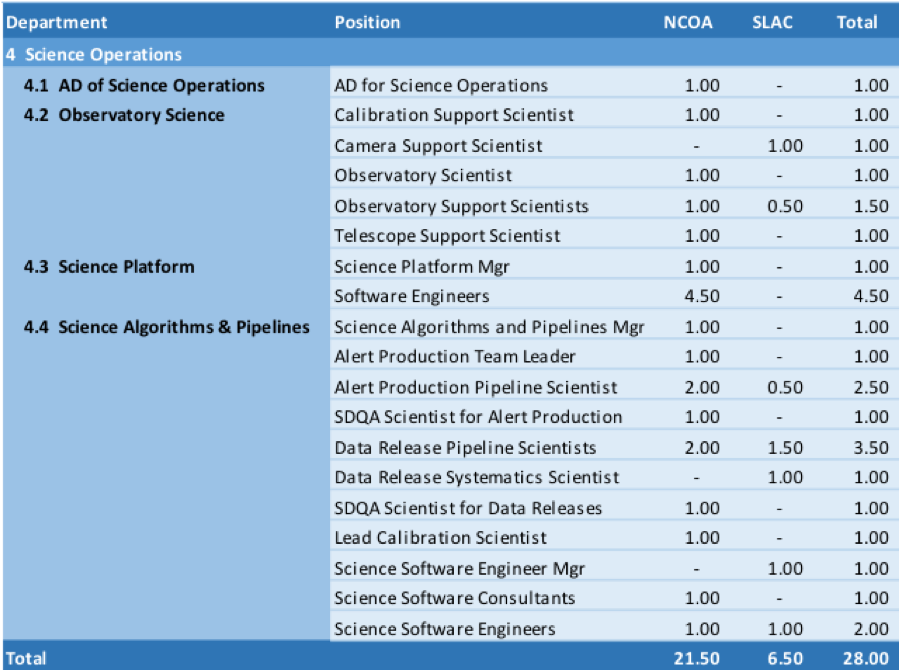
\includegraphics[width=\textwidth]{SciOpsFTE}
\end{column}
\end{columns}

}


\frame{\frametitle{ Large Data Facility}

\vspace{10pt}
\begin{columns}
\begin{column}{0.4\textwidth}
\vspace{-5.5cm}
\\
NCSA scientific and technical staff drawn from existing core areas of Center expertise. \\
\vspace{15pt}
FNAL due to proximity and existing collaborative relationships (e.g., DES). \\
\vspace{15pt}
SLAC due to intimate knowledge of software created during the LSST construction project. Currently includes QSERV\\


\end{column}
\begin{column}{0.6\textwidth}
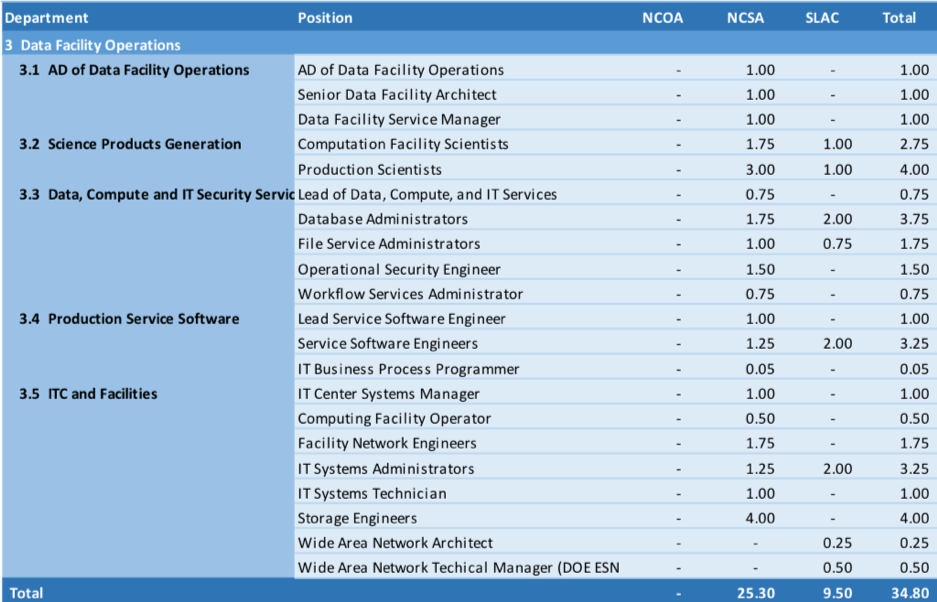
\includegraphics[width=\textwidth]{LDFFTE}\\
\end{column}
\end{columns}

}



\frame{\frametitle{Operations Rehearsals }
\tiny
\begin{longtable} {|l|l|p{0.7\textwidth}|}
	\hline
\textbf{Date/Freq} &\textbf{Location}& \textbf{Title, Description} \\ \hline

Oct 2018 &  NCSA & \textbf{Operations rehearsal for commissioning }
	With TBD weeks commissioning (lets say a week) -- pick which parts of plan we could rehearse.
	Chuck suggests Instrument Signal Removal should be the focus of this (or the next rehearsal).
	\\ \hline
Oct 2019 & NCSA &  \textbf{Operations rehearsal \#2 for commissioning}
More complete rehearsal -- where do the scientist look at quality data? How do they feed it back to the Telescope ?
How do we create/update calibrations ? Exercises some of the control loops.
\\ \hline
Jan 2020 & Base  &  \textbf{Operations rehearsal \#3 for commissioning}
Dress rehearsal -- Just like it will be April for the actual commissioning.
	\\ \hline
Dec 2020 &  NCSA &  \textbf{Operations rehearsal data release processing (commissioning data)}
	Dress rehearsal -- Just like it will be April for the actual commissioning.
	\\ \hline

2021 &  NCSA &  \textbf{Operations rehearsal for data release processing (regular data).}
	\\ \hline

Feb 2022 &  NCSA/Base &  \textbf{Operations rehearsal}
Rehearsals for real operations which start Oct 2022
	\\ \hline
Sept 2022 &  NCSA/Base &  \textbf{Operations rehearsal}
Full Dress rehearsal for real operations which start Oct 2022
	\\ \hline


\end{longtable}

\normalsize
}


\frame{\frametitle{LSST Operations - Proposed Staffing profile}
\includegraphics[width=0.9\textwidth]{images/opsStaffProfile}
}
\frame{\frametitle{LSST Operations - Construction transition}
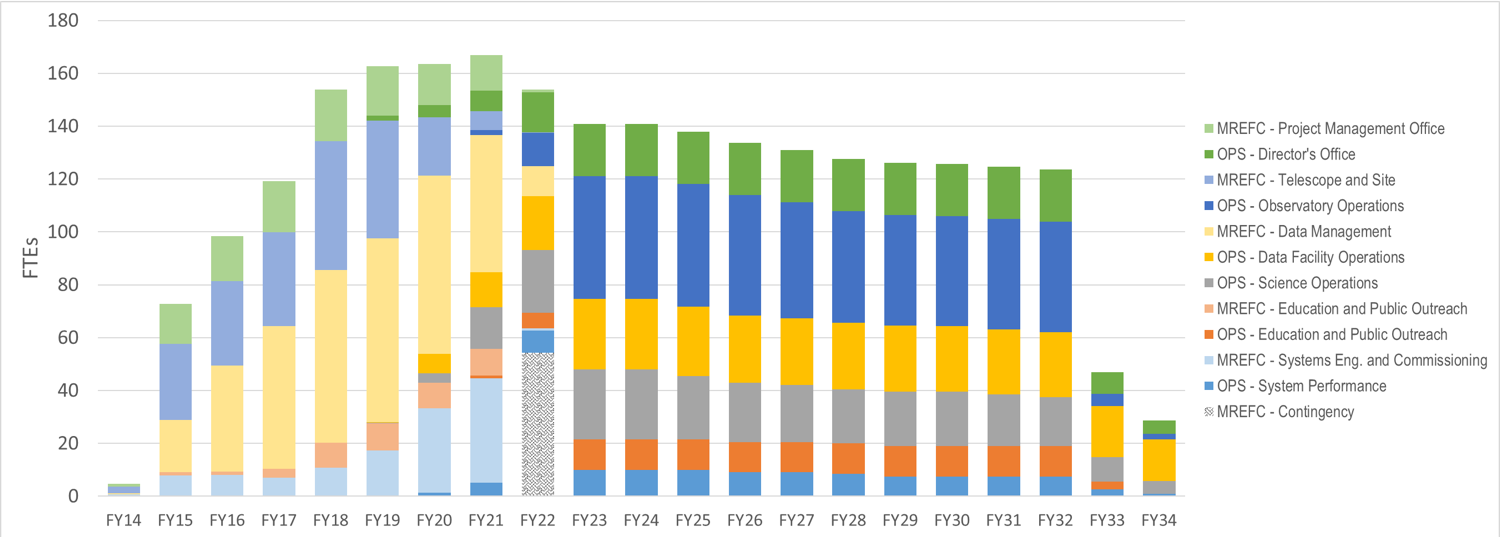
\includegraphics[width=1.0\textwidth]{opsTransFTE}
}

\section{Data Management }

\frame {\frametitle{ LSST org chart - where DM fits }
\begin{columns}
\column{0.65\textwidth}
      \includegraphics[width=1.2\textwidth]{images/Org_Chart_LSST}\\
\column{0.35\textwidth}
 \\
\vspace{-5cm}
LSST project is large and dispersed\\
Data Management  is just one of five subsystems.

\end{columns}
}


\frame {\frametitle{ Data management }
\begin{columns}
\column{0.65\textwidth}
      \includegraphics[width=1.0\textwidth]{images/DmMap}\\
\column{0.35\textwidth}
 \\
\vspace{-6cm}

 DM Mission :\\
    {\em  Stand up operable, maintainable, quality services to deliver high-quality LSST data products for science, all on time and within reasonable cost.}\\
    \vspace{14pt}
LSST DM development is distributed across the Americas.\\

{\color{blue} Plus we have partners like IN2P3}

\end{columns}
}

\frame {\frametitle{ DM Organization}
\vspace{-0.5cm}
\begin{columns}
\column{0.7\textwidth}
\begin{center}
      \includegraphics[width=1.0\textwidth]{images/DmOrg}\\
\end{center}
\column{0.3\textwidth}
 \\
\vspace{0.21cm}
DM leadership meet two times a year and have a weekly telecon. \\

Technical mangers have a {\em standup} every Tuesday and Friday. \\
{\color{red} Toughest thing in any project is communication.}
\end{columns}
}

\frame {\frametitle{  DM build and deploy }
\vspace{-1cm}
\begin{columns}
\column{0.33\textwidth}
\begin{center}
      \includegraphics[width=1.0\textwidth]{images/DMSDeployment}\\
\end{center}
\column{0.6\textwidth}
 \\
\vspace{1cm}
DM must build everything to get LSST products (see \url{http://ls.st/dpdd})  to the users.
\begin{itemize}
\item large data sets (20TB/night)
\item complex analysis
\item aiming for small systematics
\item Science Alerts in under 2 minutes .. (aiming for 1 minute)
\end{itemize}
About $1\over{2}$  million lines of code (C++/python)\\
\vspace{25pt}
{\tiny diagram K.T. Lim}
\end{columns}
}

\frame {\frametitle{  Data Backbone}
\begin{columns}
\column{0.45\textwidth}
      \includegraphics[width=1.0\textwidth]{images/DataBackbone}\\
\column{0.55\textwidth}
 \\
 \vspace{-6cm}
 One small box on the previous slide was Data Backbone.\\ That hides several things \\
 \begin{itemize}
 \item Qserv - the LSST end user database
\item All the networks : we now have fiber to the mountain and from La Serena to NCSA (two routes)
 \end{itemize}
\vspace{25pt}
{\tiny diagram K.T. Lim}
\end{columns}
}


\frame {\frametitle{Data flow }
\begin{columns}
\column{0.65\textwidth}
      \includegraphics[width=1.0\textwidth]{images/NearRealTimeDataFlow}\\
\column{0.35\textwidth}
\\
\vspace{-7cm}
Lots to do every night ..\\
Plus annually there is a data release \\
      \includegraphics[width=1.0\textwidth]{images/AnnualReprocessingDataFlow}\\

      {\tiny Images from K.T. Lim}
\end{columns}
}

\frame {\frametitle{All comes down to images \ldots }
\vspace{-5mm}
\begin{columns}
\column{0.45\textwidth}
\vspace{-2mm}
\begin{center}
      \includegraphics[width=1.0\textwidth]{images/ImSim-2011-half}\\
\end{center}
\column{0.5\textwidth}
 \\
\vspace{1cm}
False color from 3 simulated filter images\\
{\color{red} From just one of 109 CCDs}\\
\vspace{3mm}
To work with that there is the {\em LSST Stack} \url{https://pipelines.lsst.io/}\\
Current version 14.0 release in November 2017.\\
Python 3 and C++ 14.
\end{columns}
}






\frame{\frametitle{Science Platform Vision to Reality }
\vspace{-5pt}
Vision: \citeds{LSE-319} --- Design: \citeds{LDM-542} --- Test: \citeds{DMTR-51} at NCSA

\begin{columns}
\begin{column}{0.7\textwidth}
\includegraphics[width=1\textwidth]{images/psfnb}
\end{column}
\begin{column}{0.3\textwidth}
\vspace{-7cm}
\\
Portal/Browser\\
Notebooks\\
Web API\\
(Batch)\\
\hspace{-1.5cm} \includegraphics[width=1.3\textwidth]{images/firefly}\\
\hspace{0.1cm} {\tiny \bf Images Krughoff($\leftarrow$) and Wu ($\uparrow$)}
\end{column}
\end{columns}

}


\frame {
  \frametitle{ Evolution of the platform}

\begin{itemize}
\item Documentation
\begin{itemize}
\item  The direction is now documented in \citeds{LSE-319}
\item More formal requirements in \citeds{LDM-554}
\item Design is in \citeds{LDM-542}
\item First user reports in \citeds{DMTR-22}
\end{itemize}
\item Coming soon
\begin{itemize}
\item Portal focus on exploration/discovery of data products
\item full sky browsing e.g. something like HiPS \url{http://www.ivoa.net/documents/HiPS/}
\item Authentication integrated with existing credentials
\item Quotas on CPU and Disk .. has to be done..
\item Data Upload to user space
\item Scheme to include collaborator code in Stack (thus in platform)
\begin{itemize}
        \item proper way to pull any module or code into notebook kernel from say github
\end{itemize}
\end{itemize}
\item To be used in commissioning by the commissioning team
\begin{itemize}
\item Boot camps soon
\end{itemize}
\end{itemize}

}



\frame{\frametitle{Preparing for LSST: Science Collaborations }
\begin{itemize}
\item 9 LSST science collaborations, covering the science topics envisioned for LSST:
\begin{itemize}
\item AGN; Dark Energy; Galaxies; Stars, Milky Way and Local Volume; Solar System; Statistics and Informatics; Strong Lensing; Supernovae; Transients/Variable Stars
\end{itemize}
\item Preparing the LSST for the community, and the community for LSST
\item More than 400 unique members!
\end{itemize}
\begin{columns}

\column{0.85\textwidth}
{\color{red} \bf All Contributors with data rights can join !}\\
Initial collaboration work: LSST Science Book\\ \citep{scibook}
\column{0.15\textwidth}
\hfill \vspace{-1cm} \includegraphics[width=1\textwidth]{images/scibookcover}
\end{columns}
}

\section {Conclusion}
\begin{frame}{Conclusion}

\begin{itemize}
\item Current astronomical surveys are changing the way we do astronomy
\item LSST will soon follow perhaps ushering a complete change in how we approach end
user data interaction
\item LSST is on track and data is coming sooner than you might think
\item There are plenty of challenges
\item Verification and Validation on radar for now
\item Looking forward to the first LSST images !


\end{itemize}

\vspace {10pt}
Motto for the future from LSST Project Scientist:
\begin {center}
{\color{blue}   Ask Not What Data You Need To Do Your Science,\\ Ask What Science You Can Do With Your Data. }\\
\hfill {\tiny \bf \u{Z}eljko Ivezi\'c}
\end {center}
\end{frame}



\frame {
  \frametitle{ The END }
\vspace{-0.3cm}
\begin{center}
 \includegraphics[width=0.4\textwidth]{images/SDSScosmos}
\hfill
 \includegraphics[width=0.4\textwidth]{images/HSCcosmos}
\vspace{-3cm}\hspace{1cm} \huge{\color{red} Questions?}\\
\vspace{+2.0cm}
\normalsize
{$\sim  3.5 \arcmin$ SDSS image   \hfill  HSC image (COSMOS)   \\\hfill \tiny g,r(1.5 hrs) ,i(3 hrs) PSF matched co-add ($\approx 27.5$)\\}

\vspace{-5pt}
{\tiny \url{http://www.lsst.org}} {\tiny \url{http://community.lsst.org}} \hfill
{\tiny Images:Lupton and HSC colaboration see also \cite{2004PASP..116..133L}}
\end{center}

}



\appendix
\section {Reference material}
\frame[allowframebreaks]{\frametitle{ Acronyms }
	\vspace{10pt}
	\tiny
	\addtocounter{table}{-1}
\begin{longtable}{|l|p{0.8\textwidth}|}\hline
\textbf{Acronym} & \textbf{Description}  \\\hline

AURA&Association of Universities for Research in Astronomy \\\hline
C&Specific programming language (also called ANSI-C) \\\hline
DM&Data Management \\\hline
ESA&European Space Agency \\\hline
ESAC&European Space Astronomy Centre (VilSpa) \\\hline
ESOC&European Space Operations Centre (ESA) \\\hline
ESTEC&European Space research and TEchnology Centre (ESA) \\\hline
HEALPix&Hierarchical Equal-Area iso-Latitude Pixelisation \\\hline
HTM&Hierarchical Triangular Mesh \\\hline
LSST&Large Synoptic Survey Telescope \\\hline
PhD&Doctorate in Philosophy \\\hline
SDSS&Sloan Digital Sky Survey \\\hline
TEC&Thermo-Electric Cooler \\\hline
USA&United States of America \\\hline
arcmin&arcminute, minute of arc (unit of angle) \\\hline
arcsec&arcsecond, second of arc (unit of angle) \\\hline
\end{longtable}

}

\frame{\frametitle{ References }
	\tiny
	\bibliographystyle{lsst_aa}
	\bibliography{local,lsst,gaia_livelink_valid,refs,books,refs_ads}
	\normalsize

}
%\section {Backup slides}

\end{document}
